\documentclass[a4paper,12pt]{article}

% Layout
\usepackage[a4paper, left=2.5cm, right=2cm, top=1cm, bottom=3cm]{geometry} % kleinere Ränder
\usepackage{parskip}

\usepackage{fontspec}
\usepackage{lmodern}
\usepackage[english]{babel}

% Mathesymbole und Ähnliches
\usepackage{amsthm}
\usepackage{amsmath}
\usepackage{mathtools}
\usepackage{amssymb}
\usepackage{bussproofs}		% Sequenzenkalkül
\usepackage{xcolor}

% Grafiken und PDFs einfügen
\usepackage{pdfpages}
\usepackage{float}

% PDF-Tools
\usepackage[hidelinks, unicode]{hyperref}

% Abbildungen
\usepackage{tikz}
\usetikzlibrary{arrows,calc,positioning}
\tikzset{ 
   state/.style={circle,fill,inner sep=2pt,label=below:#1\strut},
   arrow/.style={->, shorten <=3pt, shorten >=3pt, >=stealth',thick},
   knoten/.style={draw, circle, minimum size=8mm}} 
   

% Reelle, Natürliche, Ganze, Rationale Zahlen
\newcommand{\R}{\ensuremath{\mathbb{R}}}
\newcommand{\N}{\ensuremath{\mathbb{N}}}
\newcommand{\Z}{\ensuremath{\mathbb{Z}}}
\newcommand{\Q}{\ensuremath{\mathbb{Q}}}
\newcommand{\C}{\ensuremath{\mathbb{C}}}
\newcommand{\B}{\ensuremath{\mathbb{B}}}
\newcommand{\F}{\ensuremath{\mathbb{F}}}


% Körper
\newcommand{\K}{\ensuremath{\mathcal{K}}}
%\newcommand{\G}{\ensuremath{\mathcal{G}}}

% Makros für logische Operatoren
\newcommand{\xor}{\ensuremath{\oplus}} % exklusives oder
\newcommand{\impl}{\ensuremath{\rightarrow}} % logische Implikation
\newcommand{\Lor}{\ensuremath{\bigvee}}
\newcommand{\Land}{\ensuremath{\bigwedge}}
\newcommand{\Eq}{\ensuremath{\Leftrightarrow}}
\newcommand{\mal}{\ensuremath{\cdot}}

% Meistens ist \varphi schöner als \phi, genauso bei \theta
\renewcommand{\phi}{\varphi}
\renewcommand{\theta}{\vartheta}

\newcommand*{\todo}{\textbf{\textcolor{red}{TODO}}}		% big, red, apparent TODO

% SEQUENZENKALKÜL
\newcommand{\yields}{\ensuremath{\mathrel{\Rightarrow}}}

% Aufzählungen anpassen (alternativ: \arabic, \alph)
\renewcommand{\labelenumi}{(\roman{enumi})}

% BITTE NICHT ÄNDERN: interne Kommandos für die Informationen (Blattnummer, Gruppe, ...)
\newcounter{sheet}
\newcommand{\printsheet}{\arabic{sheet}}


\newcommand{\printgroup}{?}
\newcommand{\group}[1]{%
\renewcommand{\printgroup}{#1}%
}

\newcommand{\printmembers}{}
\newcommand{\printmember}[3]{{#2} {#3} & {#1} \\}

\newtheorem{proposition}{Proposition}[sheet]

% Für Vektoren
\newcommand{\myvec}[1]{\ensuremath{\begin{pmatrix}#1\end{pmatrix}}}
\def\spvec#1{\left(\vcenter{\halign{\hfil$##$\hfil\cr \spvecA#1;;}}\right)}
\def\spvecA#1;{\if;#1;\else #1\cr \expandafter \spvecA \fi}

\newcommand{\pdfmembers}{}
\newcommand{\pdfmember}[3]{{#1} {#3}, {#2}; }

\newcommand{\member}[3]{%
\expandafter\renewcommand\expandafter\printmembers\expandafter{\printmembers\printmember{#1}{#2}{#3}}%
\expandafter\renewcommand\expandafter\pdfmembers\expandafter{\pdfmembers\pdfmember{#1}{#2}{#3}}%
}

\AtBeginDocument{\hypersetup{
    pdftitle = {Sheet \printsheet},
    pdfauthor = {Group \printgroup: \pdfmembers},
    pdfsubject = {Concurrency Theory}
}}

% <-------- HIER alle Informationen eintragen ========================
\setcounter{sheet}{3} % Nummer des Blatts

% alle Gruppenmitglieder in der Form \member{Matrikelnummer}{Vorname}{Nachname}
\member{5481114}{Danje}{Petersen}
\member{5174511}{Marc}{Majohr}

\begin{document}

% Kopfzeile
{\raggedright
\begin{tabular}{l}
    Concurrency Theory \\
    SS 2024 \\
    \today{} \\
\end{tabular}}
\hfill
{\Large Sheet 0\printsheet}
\hfill
\begin{tabular}{l l}
\printmembers
\end{tabular}
\hrule


% <-------- HIER beginnt die Lösung ========================

\section*{Aufgabe \printsheet.1} \setcounter{section}{1}
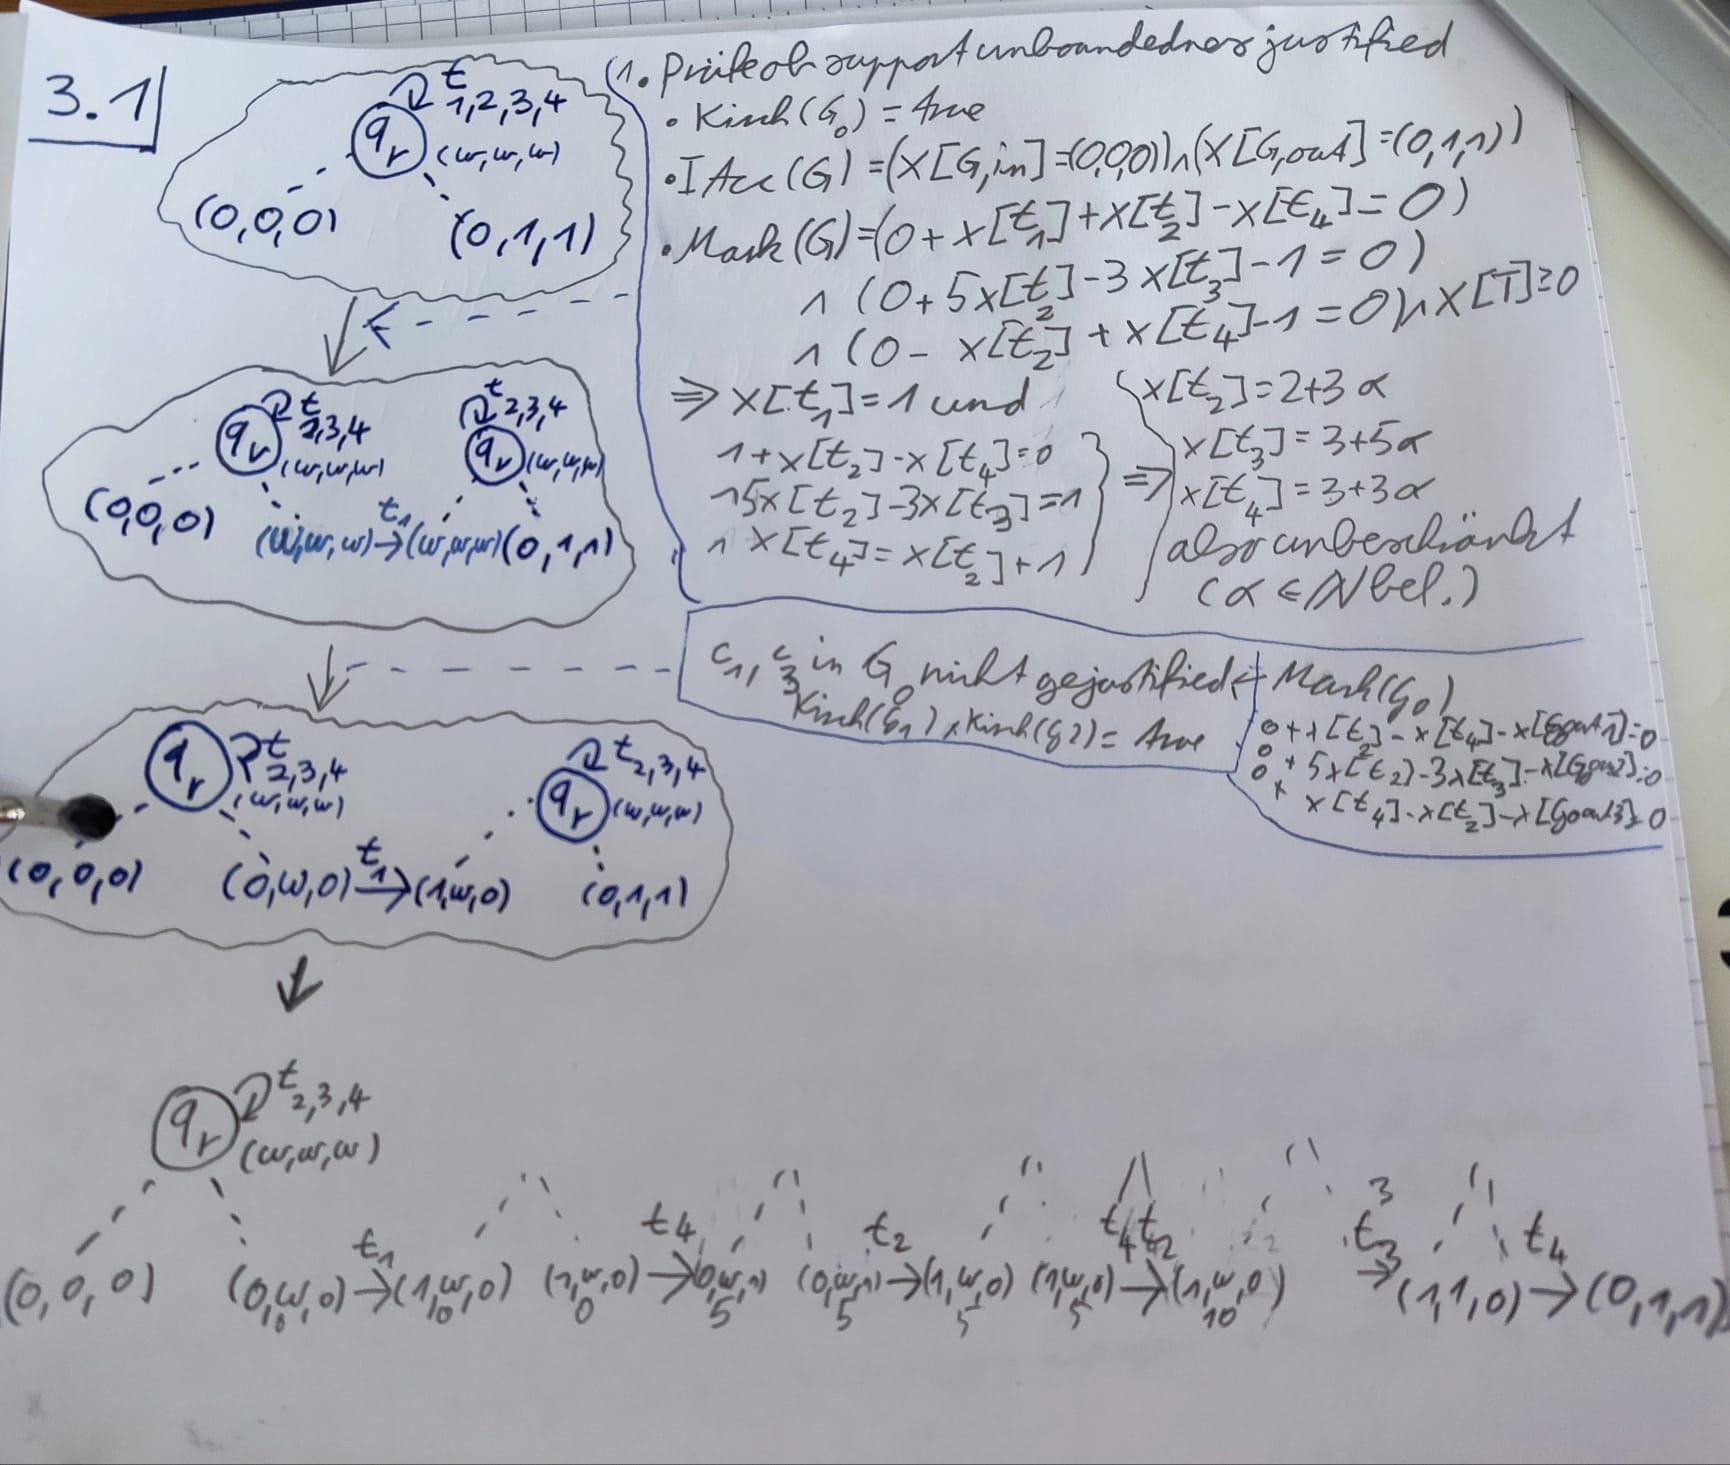
\includegraphics[scale=0.25]{1}
\section*{Aufgabe \printsheet.2}
As $a ^ {10}$ reaches  $\myvec{1&0&10&0}^T$ from $M_0=\myvec{1&0&0&0}^T$, 10 is an upper bound for the length of the shortest 3-bounded $\land$ 3-covering sequence in $(M_0,N)$.
Furthermore counter 3 is only supplied by a, therefore to achieve an increment of 10, a has to be fired at least 10 times. Therefore $|\sigma| = 10 $ is also a lower bound, thus
\textbf{m(3,M\textsubscript{0})=10}\\
Though induction (trivial) the following can be shown, where $op_3$ describes the restriction of an operation to the first 3 elements.\\
$\forall M_x,M_y\in \mathbb{Z}^S ,\sigma \ \in T^S  : (M_x \leq_3 M_y) \implies  (M_x[\sigma]_3 \implies M_y[\sigma]_3)$\\
Therefore the set of 3-bounded and 3-covering words for a Marking $M_x \leq M_y$ is a subset of the 3-bounded 3-covering words for $M_y$.
Therefore $m(3,M_x) \geq m(3,M_y)$.
As a result we only have to account for the set of smallest feasible markings (which achieve cover).
We see that (0,0,0,0) is not a viable candidate, we try m(3,(1,0,0,0)) = 10.
 The next viable candidate (after (0,1,0,0),(0,0,1,0),(0,0,0,1) which allows firing a transition is (0,1,1,1) but that immediatly results in a lower marking (0,1,0,0) which achieves no paths. \textbf{ f(3)=10}.

\section*{Aufgabe \printsheet.3}
\subsection*{(a)}
\begin{proposition} Let $N=(S,T,W,M_0)$ be a Petri net with $M_0 \in \N^n$ as the initial marking. $N$ is unbounded $\Eq$ $\exists \sigma_1,\sigma_2 \in T^*: M_0 \left[ \sigma_1 \right\rangle M_1 [ \sigma_2 \rangle M_2$ and $M_1 < M_2$. \end{proposition}
\begin{proof}
We show equality by showing implication in both directions.
\begin{itemize}
\item[$\Leftarrow$:] Assume, $\exists \sigma_1,\sigma_2 \in T^*: M_0 \left[ \sigma_1 \right\rangle M_1 [ \sigma_2 \rangle M_2 \land M_1 < M_2$ and $N$ is bounded. In this case, the set of reachable markings is finite and there must be markings $M_s$ for each place $s\in S$ in which the place has the most tokens compared to the other markings.\\ 
Let $k$ be a place in which $M_2$ has more tokens than $M_1$. Such a place must exist since $M_1 < M_2$. Since $\sigma_2$ has the effect of increasing the number of tokens at place $k$ and not decreasing the number of tokens at any other place, $\sigma_2$ can be  fired infinitely often, thus increasing the number of tokens arbitrarily. This contradicts the existence of $M_k$.
\item[$\Rightarrow$:] Assume $N$ is unbounded. The set of reachable markings must therefore be infinite. Since it was proven on Sheet 01 that a set of tuples of natural numbers is a well-quasi ordering we can assume that there must be markings $M_1$ and $M_2$ with $M_1 \leq M_2$. Since in the set of reachable markings, these markings are unique, $M_1 \neq M_2$ holds and therefore $M_1 < M_2$. Since these markings are in the set of reachable markings it is obvious that $\sigma_1$ and $\sigma_2$ as defined before must exist.
\end{itemize}
\end{proof} 

\subsection*{(b)}


\section*{Aufgabe \printsheet.4} 
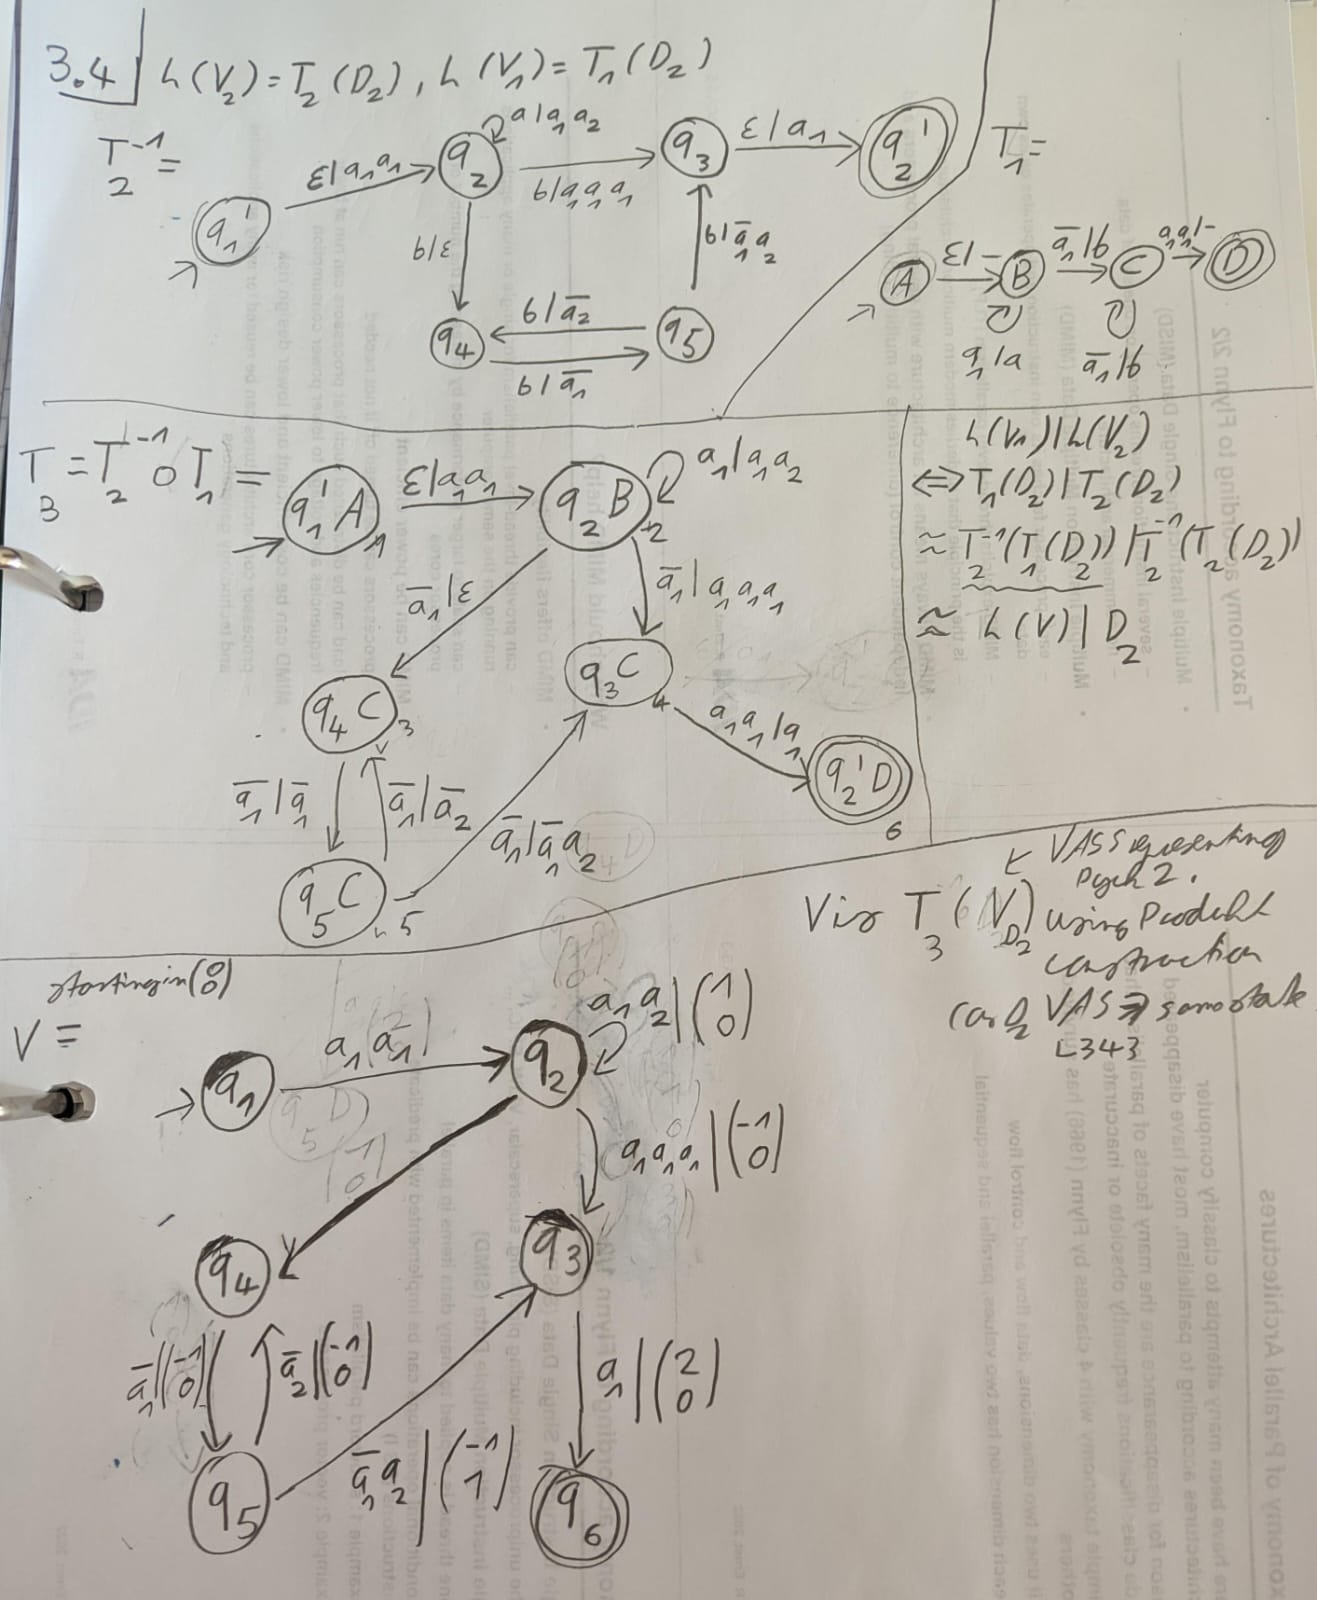
\includegraphics[scale=0.35]{4}





\end{document}
